\subsection{Balance and Stability}\label{sec:sec:balance}
Each of the methods used have to be stable through the motion in order for the system to be stable (i.e. not to fall down).  The well known zero-moment-point (ZMP) criteria is what each method must adhere to in order to stay statically stable\cite{Vukobratovic19721}.  To handle perturbation an active balance controller was added.  The active balance controller is applied on top of the pre-defined trajectories.  The Hubo is modeled as a single inverted pendulum with the center of mass (COM) located at length $L$ from the ankle.  The compliance of the robot is composed of a spring $K$ and a damper $C$, see Fig.~\ref{fig:invPen}.  An IMU located at the COM gives the measured orientation.

\begin{figure}[t]
  \centering
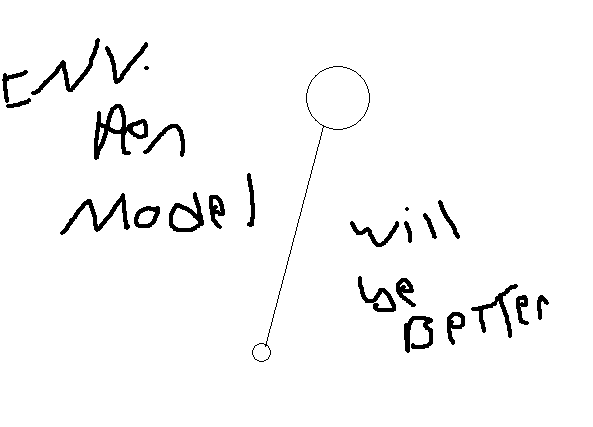
\includegraphics[width=1.0\columnwidth]{./pix/invPen.png}
  \caption{Hubo modeled as a single inverted pendulum with COM located a distance $L$ from }
  \label{fig:invPen}
\end{figure}

The dynamic equation of the simplified model is assumed to be the same in both the sagittal and coronal plane.

\begin{equation}
mL^2\ddot{\theta}+C\dot{\theta}-K\theta = Ku
\end{equation}

This can be linearized and made into the transfer function:

\begin{equation}
%G(s) = \frac{\Theta(s)}{U(s)} = \frac{K}{ mL^2s^2 + Cs + (K - mgL)}
G(s) = \frac{\Theta(s)}{U(s)} = \frac{\frac{K}{mL^2}}{s^2+\frac{C}{mL^2}s + \frac{K-mgL}{mL^2}}
\end{equation}

Prior work on the model and controller for the Hubo by Cho et. al. calculated $K=753\frac{Nm}{rad}$ and $C=18\frac{Nm}{sec}$ using the free vibration response method\cite{5379574}.


\begin{figure}[ht]
  \centering
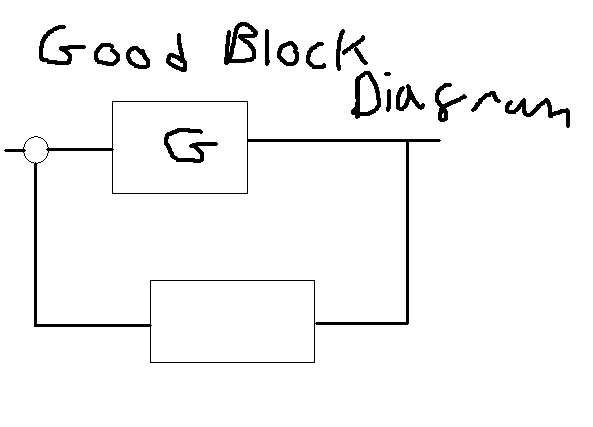
\includegraphics[width=1.0\columnwidth]{./pix/blockDiagram.png}
  \caption{Hubo successfully throwing the first pitch at the second annual Philadelphia Science Festival event Science Night at the Ball Park on April 28th, 2012.  The game was between the Philadelphia Phillies and the Chicago Cubs and played at the Major League Baseball stadium Citizens Bank Park.  The Phillies won 5-2}
  \label{fig:ctrlBlockDiagram}
\end{figure}

The control law is as follows
%ffFor the ankle roll (in the coronal plane) it is always assumed that the desired orientation of the COM is zero degrees.  Thus the roll of the IMU is taken as the error.

\begin{equation}
\theta_{n}^x = \theta_{t}^x + \left(K_p^x+sK_d^x\right)\left(\sum \theta_{t}^x - \theta_{c}^x\right)
%\theta_{n}^x = \theta_{t}^x + (K_p^x+sK_d^x)(\sum \theta_{t}^x - \theta_{c}^x)
%\theta_{new} = \theta_{traj} + (K_p+sK_d)(\sum \theta_{leg} - \theta_{IMU})
\end{equation}

Where $\theta_t$ is the desired trajectory of the lower body (pitch or roll) and $x$ denotes pitch or roll.  $\theta_{c}$ is the orientation of the center of mass in the global frame.  $\theta_n$ is the resulting trajectory.  $K_p$ and $K_d$ are the proportional and derivative gains.  The resulting control allows for a stable stance even with perturbations from upper body motions.
